\section{The Far Detector Simulation and Reconstruction}\label{sec:nu-osc-07}\label{sec:physics-lbnosc-FD}
%{\it Assigned to:} {\bf Dan Cherdack} with contributions from Nick Grant, Leigh Whitehead, Callum Wilkinson, Elizabeth Worcester and Tingjun Yang.
\label{sec:physics-lbnosc-simreco}
%This section describes assumptions in the Near Detector simulation and reconstruction. Some thought has to go into the connection to the Far Detector chapter in the TDR.

%\begin{itemize}
%    \item Simulations - TY 
%    \item Reconstruction and kinematic variables including energy reconstruction - TY, NG 
%    \item Event selections (CVN) - LW
%    \item Samples - EW, CW
%    \item Detector response systematic uncertainties - DDC
%    \item Connection to flux and cross section systematic uncertainties
%\end{itemize}

The calculation of \dword{dune} sensitivities to oscillation parameter measurements requires predictions for the number of events to be observed in the \dword{fd} fiducial volume, the reconstructed neutrino energy for each of these events, and the probability that they will be correctly identified as signal for each analysis samples. To build these analysis samples a  \dword{geant4} simulation of the \dword{fd} has been developed. The output of that simulation has been used to build neutrino energy estimators, and an event selection discriminant that can separate $\nu_{e}$ \dword{cc}, $\nu_{\mu}$ \dword{cc}, and \dword{nc} events. Each of these components is described in detail in this section. The uncertainties associated with each step in the simulation and reconstruction chain, including the \dword{fd} simulation, reconstructed energy estimators, and selection efficiencies are discussed in Section~\ref{sec:nu-osc-09}. 


\subsection{Simulation}
The neutrino samples were simulated using a smaller version of the full \nominalmodsize far \dword{detmodule} geometry. This geometry is 13.9 m long, \tpcheight high and 13.3 m wide, which consists of 12 \dwords{apa} and 24 \dwords{cpa}. The reference flux was used (Section~\ref{sec:physics-lbnosc-flux}) and samples were produced with both the forward-horn-current (neutrino enhanced) and inverted-horn-current (antineutrino enhanced) beam configurations. Three samples were generated. The first sample keeps the original neutrino flavor composition of  the neutrino beam. The second sample converts all the muon neutrinos to electron neutrinos. The third sample converts all the muon neutrinos to tau neutrinos. Oscillation probabilities are used to weight \dword{cc} events to build oscillated \dword{fd} predictions from the three event samples. \dword{genie} 2.12.10 was used to model the neutrino-argon interactions in the volume of cryostat. The produced final-state (after \dword{fsi}) particles were propagated in the detector through \dword{geant4}. %{\sc geant}. Check if right!
The ionization electrons and scintillation light were digitized to produce signals in the wire planes and \dwords{pd}. More details on the simulation can be found in Section~\ref{sec:tools-mc-detsim}.

\subsection{Event Reconstruction and Kinematic Variables}
The first step in the reconstruction is to convert the raw signal from each wire to a standard (e.g., Gaussian) shape. This is achieved by passing the raw data through a calibrated deconvolution algorithm to remove the impact of the \dword{lartpc} \efield and the electronic response from the measured signal. The resulting wire waveform possesses calibrated charge information. 

The hit-finding algorithm scans the processed wire waveform looking for local minima. If a minimum is found, the algorithm follows the waveform after this point until it finds a local maximum. If the maximum is above a specified threshold, the program scans to the next local minimum and identifies this region as a hit. Hits are fit with a Gaussian function whose features identify the correct position (time coordinate), width, height, and area (deposited charge) of the hit. A single Gaussian function is used to describe hits produced by isolated single particles. In regions where there are overlapping particles (e.g., around the neutrino interaction vertex) single Gaussian fits may fail, and fits to multiple Gaussian functions may be used. The reconstructed hits are used by reconstruction and event selection pattern recognition algorithms. In particular the \dword{cvn} event selection algorithm is described later in this section.

The reconstruction algorithms (\dword{pandora} and \dword{pma}) define clusters as hits that may be grouped together due to proximity in time and space to one another. Clusters from different wire planes are matched to form high-level objects such as tracks and showers. These high level objects are used as inputs to the neutrino energy reconstruction algorithm. More details on the reconstruction can be found in section~\ref{sec:tools-fdreco}.

% Neutrino energy reconstruction

The energy of the incoming neutrino in \dword{cc} events is estimated by adding the reconstructed lepton and hadronic energies. 
If the event is selected as $\nu_{\mu}$ \dword{cc}, the neutrino energy is estimated as the sum of the energy of the longest reconstructed track and the hadronic energy. The energy of the longest reconstructed track is estimated from its range if the track is contained in the detector, and this is calibrated using simulated $\nu_{\mu}$ \dword{cc} events with true muon energies from 0.2-1.7 GeV. If the longest track exits the detector, its energy is estimated from multi-Coulomb scattering, and corrected using simulated events with true muon energies from 0.5-3 GeV. The hadronic energy is estimated from the charge of reconstructed hits that are not in the longest track, and corrections are applied to each hit charge for recombination and the electron lifetime. An additional correction is then made to the hadronic energy to account for missing energy due to neutral particles and final-state interactions, and this is done using simulated events with true hadronic energies from 0.1-1.6 GeV. The same hadronic shower energy calibration is used for both $\nu$ and $\bar{\nu}$ based on a sample of $\nu$ and $\bar{\nu}$ events.

If the event is selected as $\nu_{e}$ \dword{cc}, the energy of the 
neutrino is estimated as the sum of the energy of the reconstructed shower with the highest energy and the hadronic energy. The former is estimated from the charges of the reconstructed hits in the shower, and the latter from the hits not in the shower; the recombination and electron lifetime corrections are applied to the charge of each hit. Subsequently the shower energy is corrected using simulated events with true electron energies from 0.5-3 GeV, and the missing energy correction is applied to the hadronic energy.

The fractional residuals of reconstructed neutrino energy are shown for $\nu_{\mu}$ \dword{cc} events with contained tracks in figure \ref{fig:enresnumucont}, for $\nu_{\mu}$ \dword{cc} events with exiting tracks in figure \ref{fig:enresnumuexit} and for $\nu_{e}$ \dword{cc} events in figure \ref{fig:enresnue}. The biases and resolutions of reconstructed neutrino energy are summarized in Table~\ref{tab:ressummary}.

%\begin{figure}[h]
%    \centering
%        \includegraphics[width=0.55\textwidth]{EnergyResNue.eps}
%        \caption{Fractional residuals of reconstructed $\nu_{e}$ energy %in $\nu_{e}$ CC events}
%        \label{fig:enresnue}
%\end{figure}

\begin{figure}
    \centering
    \begin{minipage}[t]{0.3\textwidth}
        \centering
        \hspace*{-0.5in}
        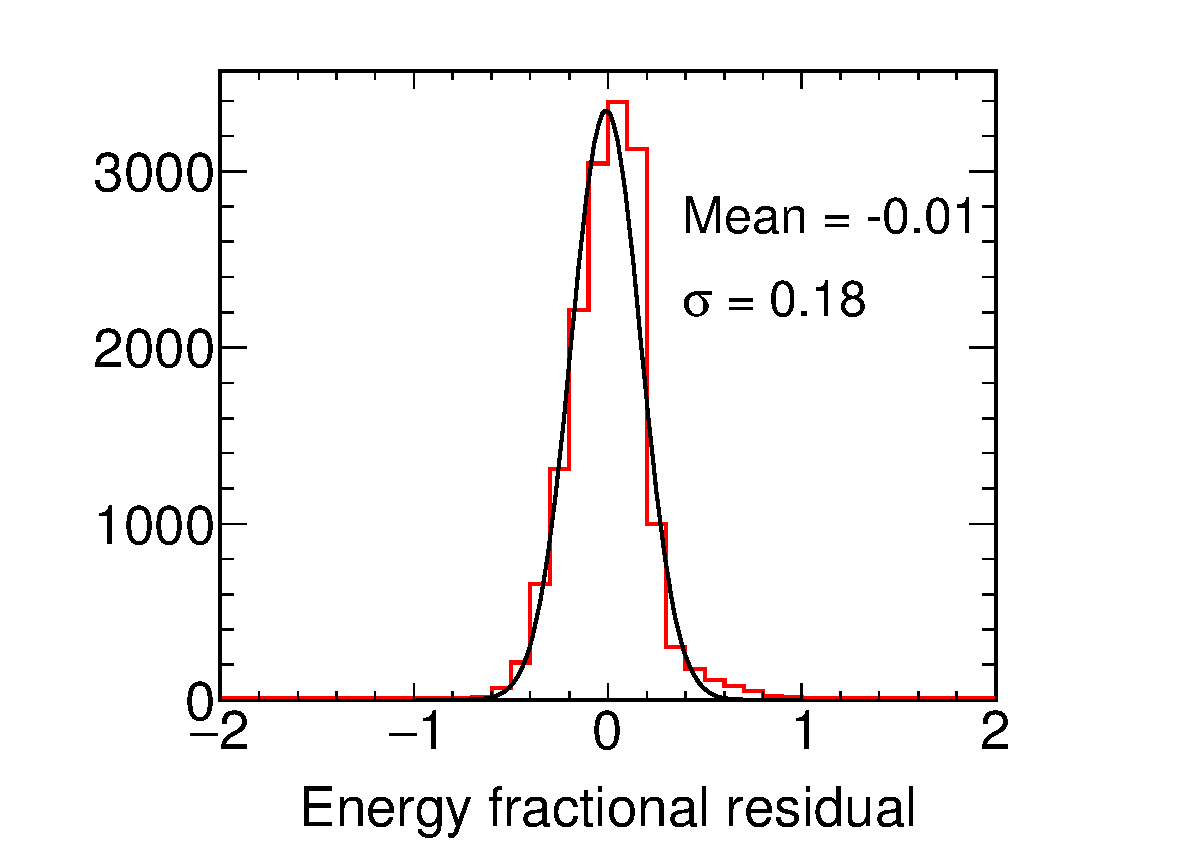
\includegraphics[width=1.37\textwidth]{EnergyResContTweak_largeFont.pdf}
        \caption[Fractional residuals of reconstructed $\nu_{\mu}$ energy in CC events with contained tracks]{Fractional residuals of reconstructed $\nu_{\mu}$ energy in $\nu_{\mu}$ \dword{cc} events with contained tracks} 
        \label{fig:enresnumucont}
    \end{minipage}\hfill
    \begin{minipage}[t]{0.3\textwidth}
        \centering
        \hspace*{-0.5in}
        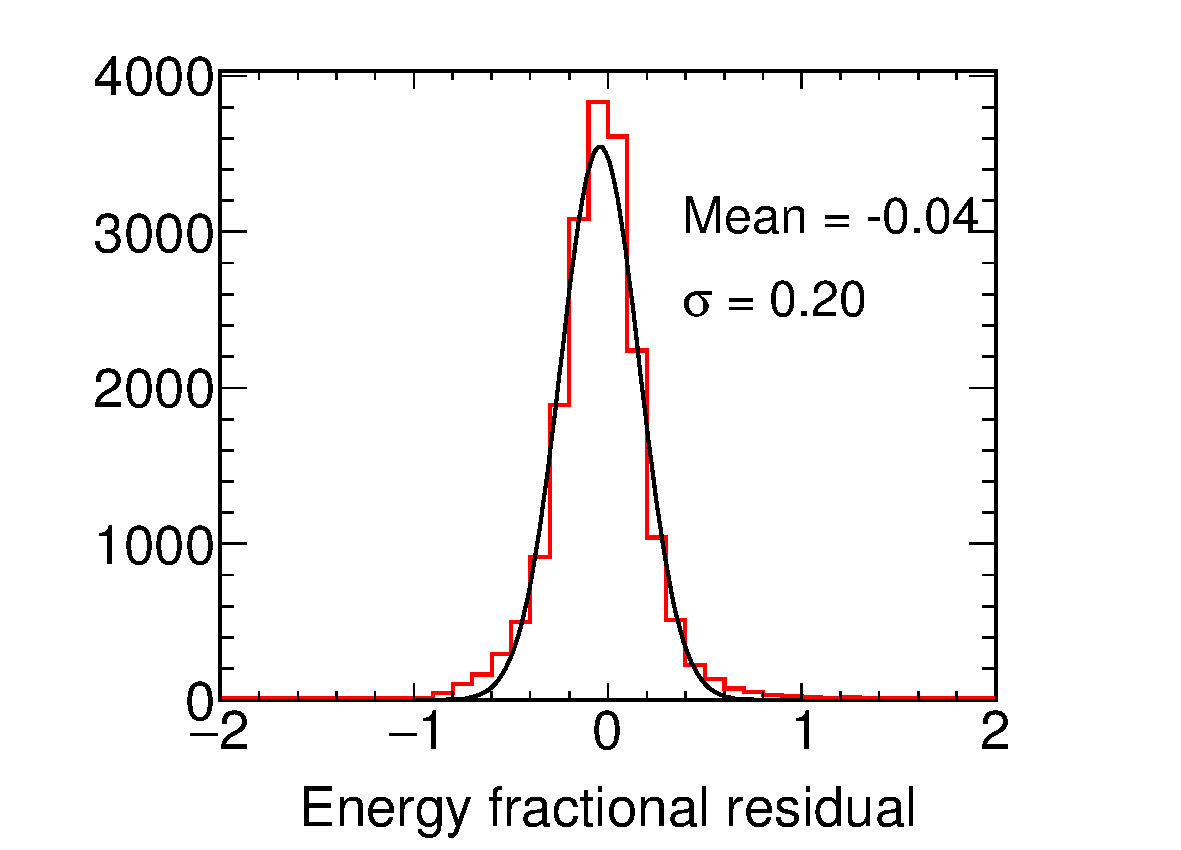
\includegraphics[width=1.37\textwidth]{EnergyResExitTweak_largeFont.pdf}
        \caption[Fractional residuals of reconstructed $\nu_{\mu}$ energy in CC events with exiting tracks]{Fractional residuals of reconstructed $\nu_{\mu}$ energy in $\nu_{\mu}$ \dword{cc} events with exiting tracks}
        \label{fig:enresnumuexit}
    \end{minipage}\hfill
    \begin{minipage}[t]{0.3\textwidth}
        \centering
        \hspace*{-0.5in}
        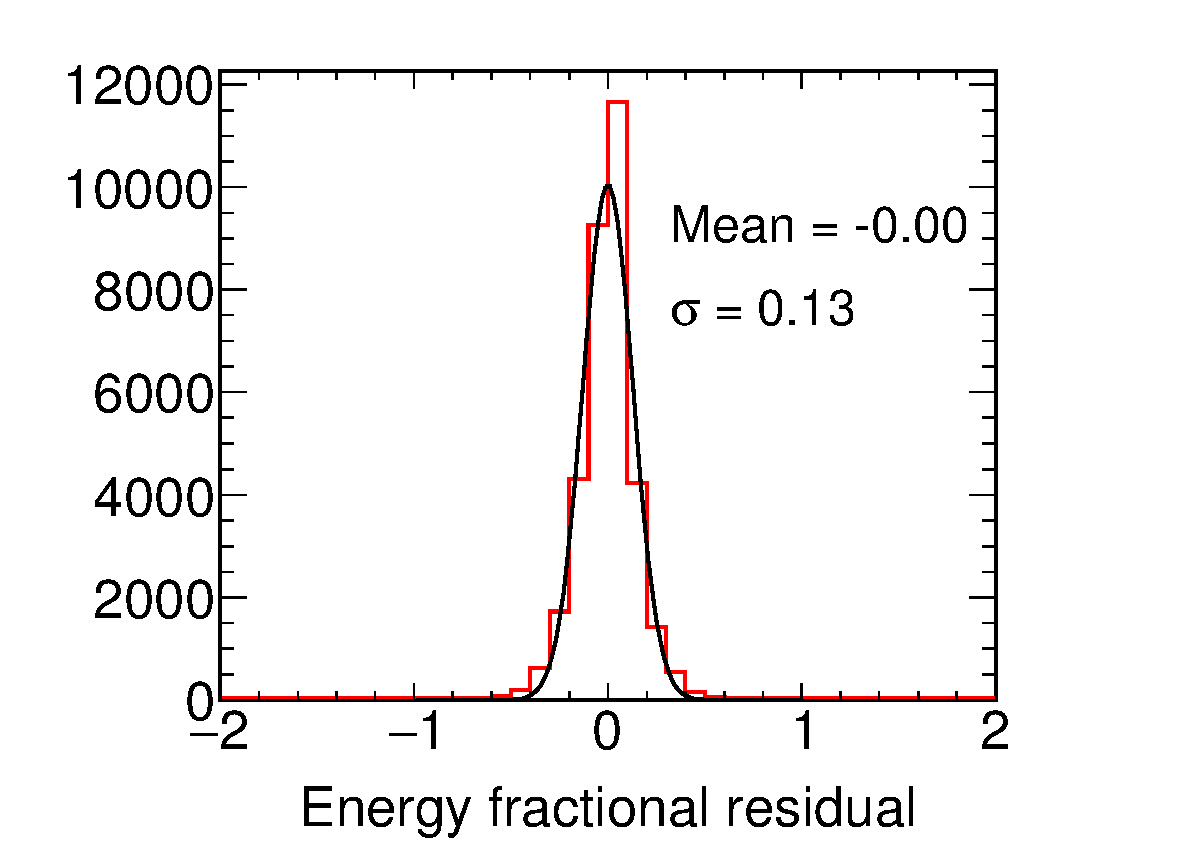
\includegraphics[width=1.37\textwidth]{EnergyResNue_largeFont.pdf}
        \caption[Fractional residuals of reconstructed $\nu_{e}$ energy in CC events]{Fractional residuals of reconstructed $\nu_{e}$ energy in $\nu_{e}$ \dword{cc} events }
        \label{fig:enresnue}
    \end{minipage}
\end{figure}

\begin{table}[h!]
\begin{center}
\begin{tabular}{|c|c|c|}
\hline  
 Event selection  &   Bias (\%) & Resolution (\%) \\ \hline
\hline
 $\nu_{\mu}$ \dword{cc} with contained track  &   -1  &  18   \\ \hline
 $\nu_{\mu}$ \dword{cc} with exiting track  &  -4   &  20 \\ \hline
 $\nu_{e}$ \dword{cc}    &  0 & 13    \\ \hline
\end{tabular}
\caption[Summary of biases and resolutions of reconstructed neutrino energy]{Summary of biases and resolutions of reconstructed neutrino energy}
\label{tab:ressummary}
\end{center}
\end{table}

% Start DUNE CVN event selection subsection from Leigh and Saul

\subsection{Neutrino Event Selection using \dword{cvn}}
The \dword{dune} \dword{cvn} classifies neutrino interactions in the \dword{dune} \dword{fd} through image recognition techniques. In general terms it is a \dword{cnn}. Similar techniques have been demonstrated to outperform traditional methods in many aspects of high energy physics~\cite{Radovic:2018dip}.

The primary goal of the \dword{cvn} is to efficiently and accurately produce event selections of the following interactions: $\nu_{\mu}$ \dword{cc} and $\nu_{e}$ \dword{cc} in the FHC beam mode, and $\bar{\nu}_\mu$ \dword{cc} and $\bar{\nu}_e$ \dword{cc} in the \dword{rhc} beam mode. Future goals will include studies of exclusive neutrino interaction final states since separating the event selections by interaction type can improve the sensitivity as interaction types have different energy resolutions and systematic uncertainties. Detailed descriptions of the \dword{cvn} architecture can be found in~\cite{Aurisano:2016jvx}.

%\subsubsection{Network architecture}
An important feature for the \dword{dune} \dword{cvn} is the fine-grained detail of a \dword{lartpc} encoded in the input images to be propagated further into the \dword{cvn}. This detail is more than what would be possible using a traditional \dword{cnn}, such as the GoogLeNet-inspired network (also called Inception v1)~\cite{GoogLeNet} used by \dword{nova}~\cite{Aurisano:2016jvx}. To accomplish this, the \dword{cvn} design is based on the SE-ResNet architecture, which consists of a standard ResNet (Residual neural network) architecture~\cite{He-et-al-2015-deep} along with Squeeze-and-Excitation blocks~\cite{Hu-et-al-2017-squeeze}. Residual neural networks allow the $n^{th}$ layer access to the output of both the $(n-1)^{th}$ layer and the $(n-k)^{th}$ layer via a residual connection, where $k$ is a positive integer ($\ge 2$).

%\subsubsection{Inputs to the \dword{cvn}}
%\label{sec:inputs}
In order to build the training input to the \dword{dune} \dword{cvn} three images of the neutrino interactions are produced, one for each of the three readout views, using the reconstructed hits on the individual wire planes. The images are not dependent on any further downstream reconstruction algorithms. The images contain 500 $\times$ 500 pixels, each in the (wire, time) parameter space, where the wire is the wire channel number and the time is the peak time of the reconstructed hit. 
%measured in \dwords{tdc}. \fixme{can you please define TDC here and we can remove it from the glossary (where it's not defined). This is the only instance of it. Or is it supposed to be TPC? Anne}
The value of each pixel represents the integrated charge of the reconstructed hit. An example simulated 2.2\,GeV $\nu_{e}$ \dword{cc} interaction is shown in all three views in Figure~\ref{fig:views} demonstrating the fine-grained detail available from the \dword{lartpc} technology.

\begin{figure}[htb] 
\centering
	\begin{tabular}{ccc}
%		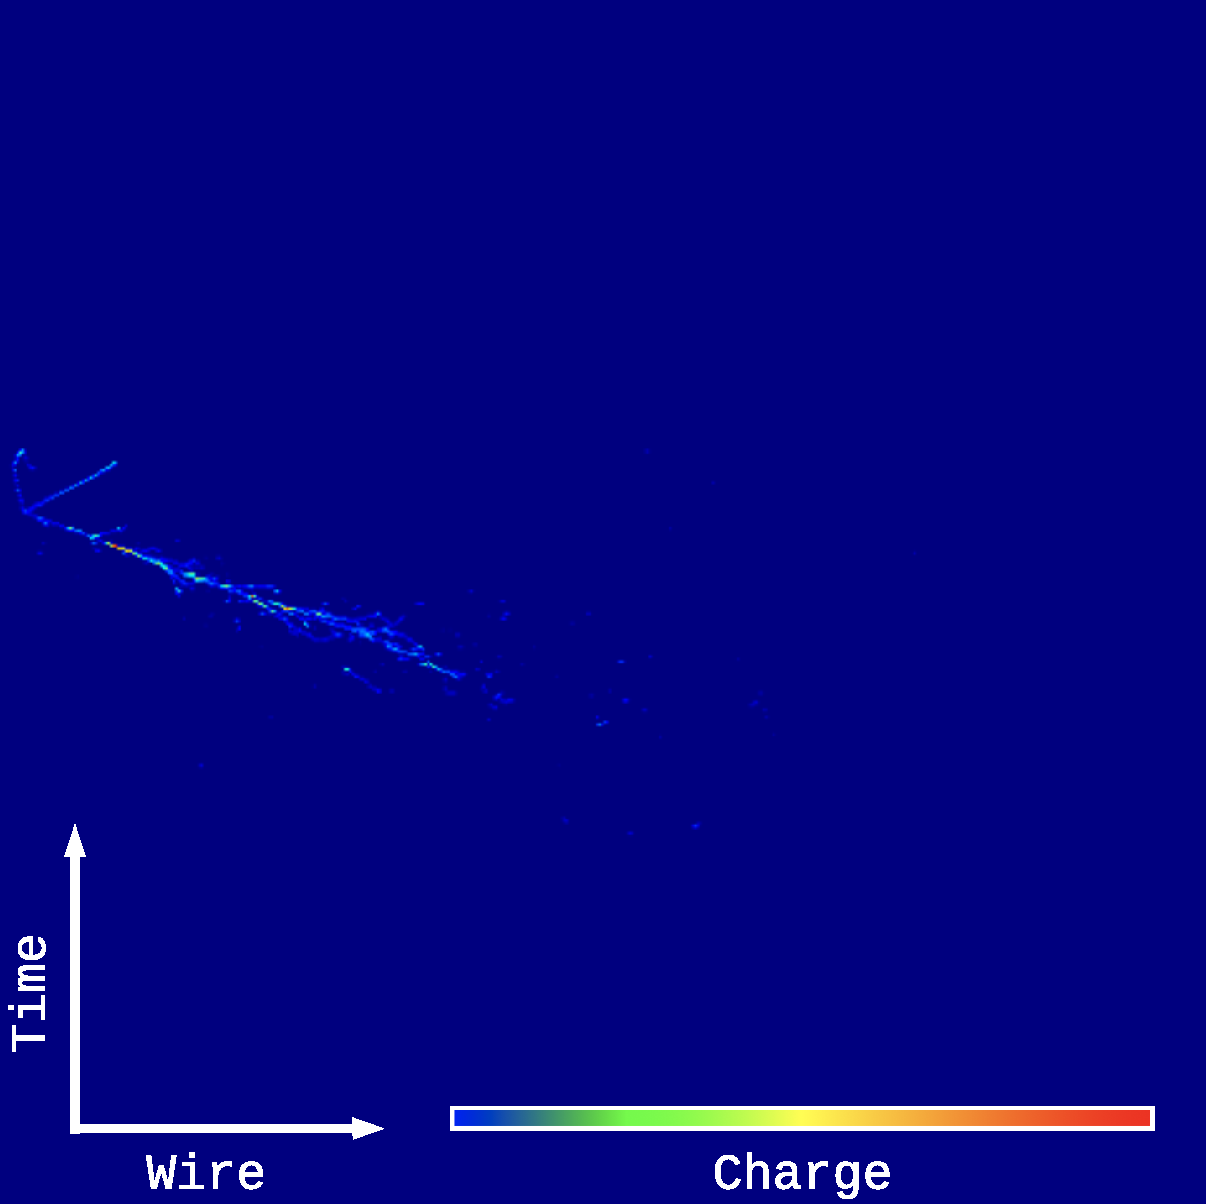
\includegraphics[scale=0.45]{cvn_nue_view0.pdf} &
%		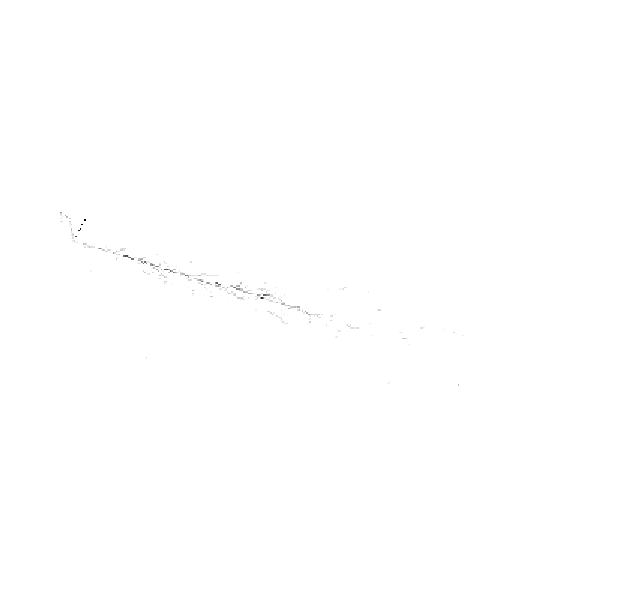
\includegraphics[scale=0.45]{cvn_nue_view1.pdf} &
		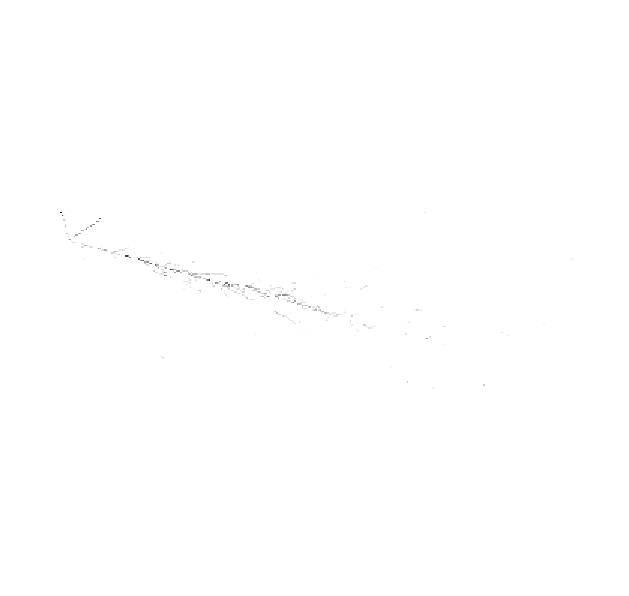
\includegraphics[trim={1cm 4cm 5cm 3cm}, clip, scale=2.0]{cvn_nue_view2.pdf}
    \end{tabular}
%	\caption{A simulated 2.2\,GeV $\nu_{e}$ \dword{cc} interaction shown in the three readout views of the \dword{dune} \dwords{lartpc}. The horizontal axis shows the wire number of the readout plane and the vertical axis shows time. The greyscale shows the charge of the energy deposits on the wires.}
\caption[A simulated \SI{2.2}{GeV} \nue CC interaction viewed by collection wires in the SP \lartpc]{A simulated 2.2\,GeV $\nu_{e}$ \dword{cc} interaction shown in the collection view of the \dword{dune} \dwords{lartpc}. The horizontal axis shows the wire number of the readout plane and the vertical axis shows time. The greyscale shows the charge of the energy deposits on the wires. The interaction looks similar in the other two views.}
	\label{fig:views}
\end{figure}

%\subsubsection{Training the \dword{cvn}}
%\label{sec:training}

The \dword{cvn} is trained using approximately three million neutrino interactions from the \dword{mc} simulation. An independent sample is used to generate the physics measurement sensitivities. The training sample is chosen to ensure similar numbers of training examples from the different neutrino flavors. Validation is performed to ensure that similar classification performance is obtained for the training and test samples, i.e., the \dword{cvn} is not overtrained.

%\subsubsection{Outputs from the \dword{cvn}}
%\label{sec:outputs}

%The \dword{cvn}, as currently constructed, has six different outputs:
%\begin{itemize}
%    \item Primary output -- neutrino flavor: returns probabilities that each interaction is one of the following classes: $\nu_{\mu}$ \dword{cc}, $\nu_{e}$ \dword{cc}, $\nu_{\tau}$ \dword{cc} and \dword{nc}.
%    \item Four particle counting outputs for protons, charged pions, neutral pions and neutrons. Probabilities are returned for the presence of 0, 1, 2 and $>2$ particles of each aforementioned type.  
%    \item Neutrino / antineutrino discriminator: returns the probability for the interaction to be an antineutrino.
%\end{itemize}

For the analysis presented here, we have used the primary output of the \dword{cvn}, namely the neutrino flavor which returns probabilities that each interaction is one of the following classes: $\nu_{\mu}$ \dword{cc}, $\nu_{e}$ \dword{cc}, $\nu_{\tau}$ \dword{cc} and \dword{nc}. 
%As stated, all of the outputs are probabilities that allow neutrino event selections to be easily defined.

\subsubsection{Neutrino Flavor Identification Efficiency}
The primary goal of the \dword{cvn} algorithm is to accurately identify $\nu_{e}$ \dword{cc} interactions and $\nu_{\mu}$ \dword{cc} interactions to allow for the selection of the samples required for the neutrino oscillation analysis. The $\nu_{e}$ \dword{cc} probability distribution, $P(\nu_e \textrm{ \dword{cc}})$, and the $\nu_\mu$ \dword{cc} probability distribution, $P(\nu_\mu \textrm{ \dword{cc}})$, are shown on the left and right of Figure~\ref{fig:cvnprob}, respectively. Excellent separation between the signal and background interactions is seen in both cases.

\begin{figure}
    \centering
    \begin{tabular}{cc}
		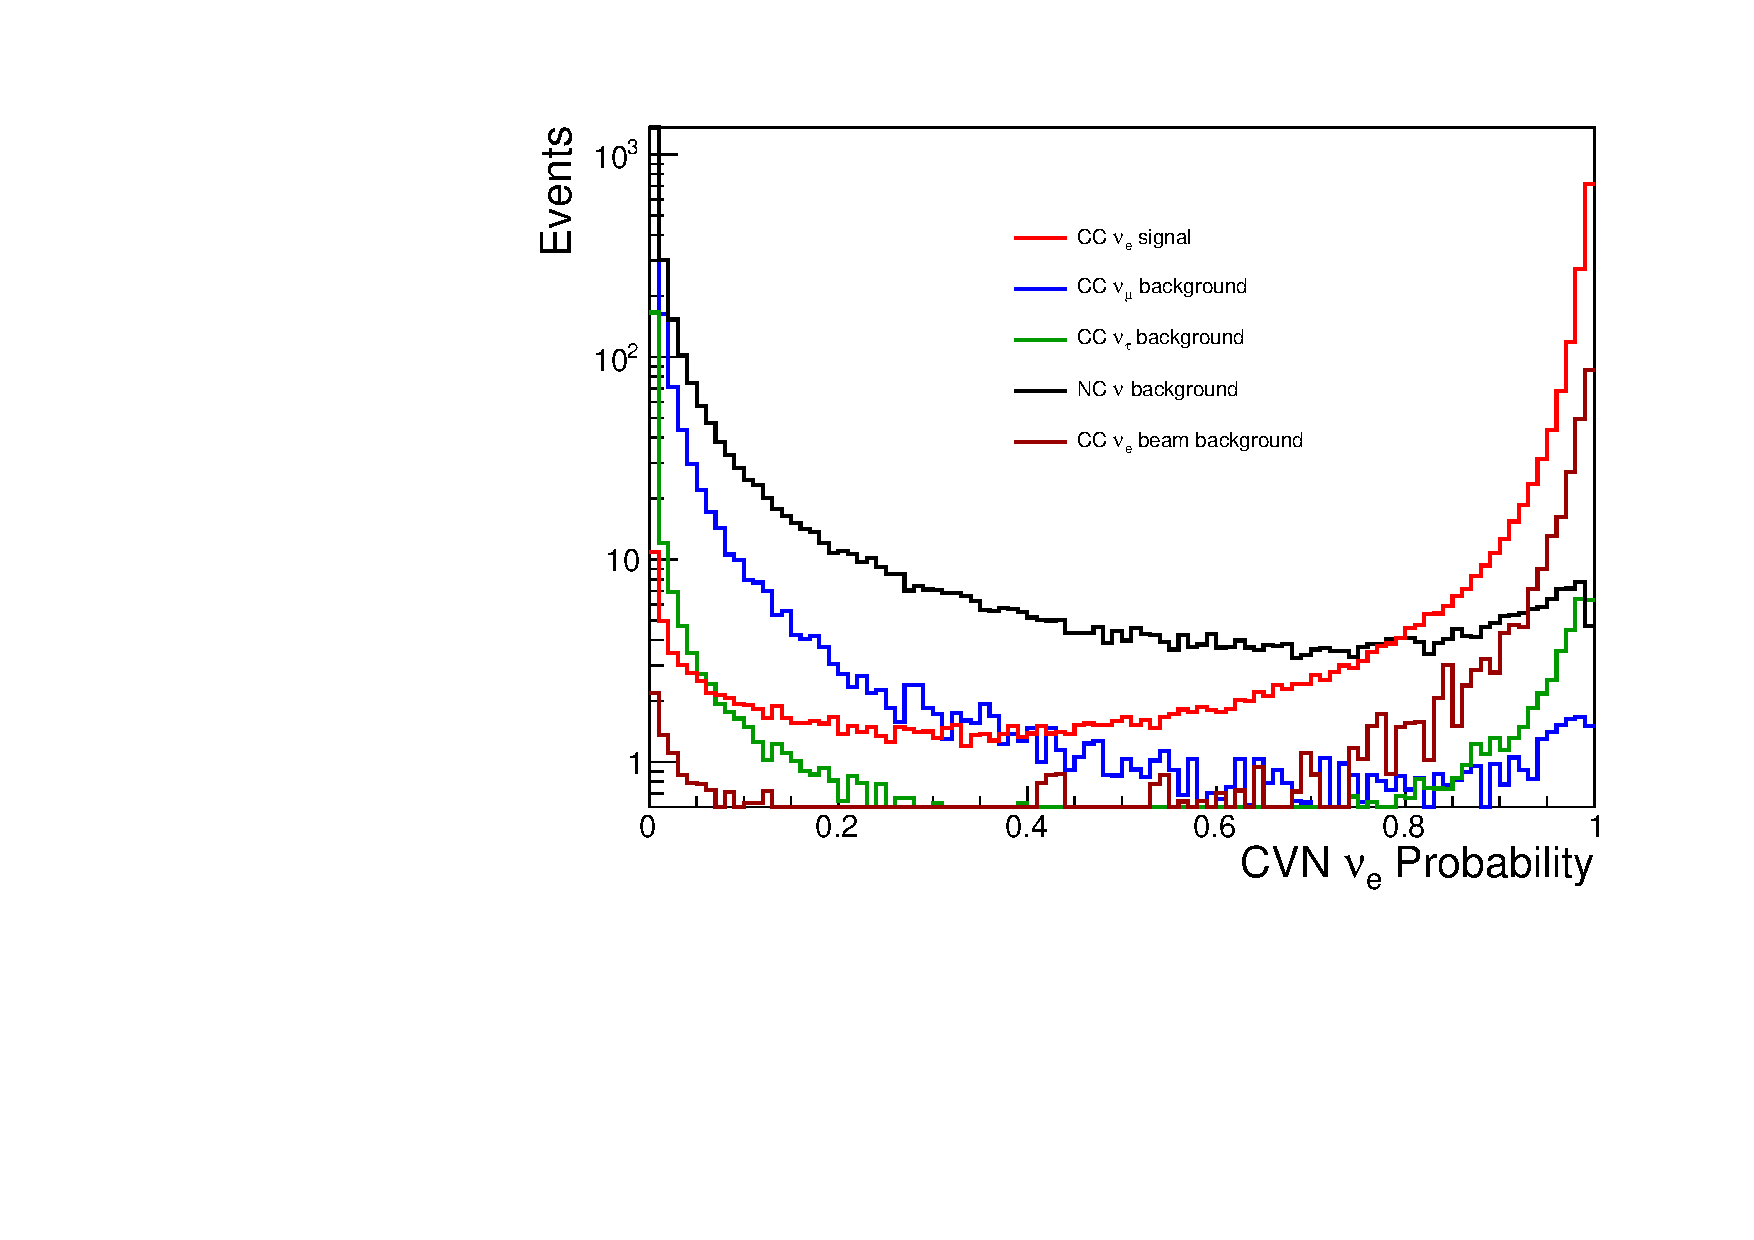
\includegraphics[width=0.45\linewidth]{cvn_nue_prob_log.pdf} &
		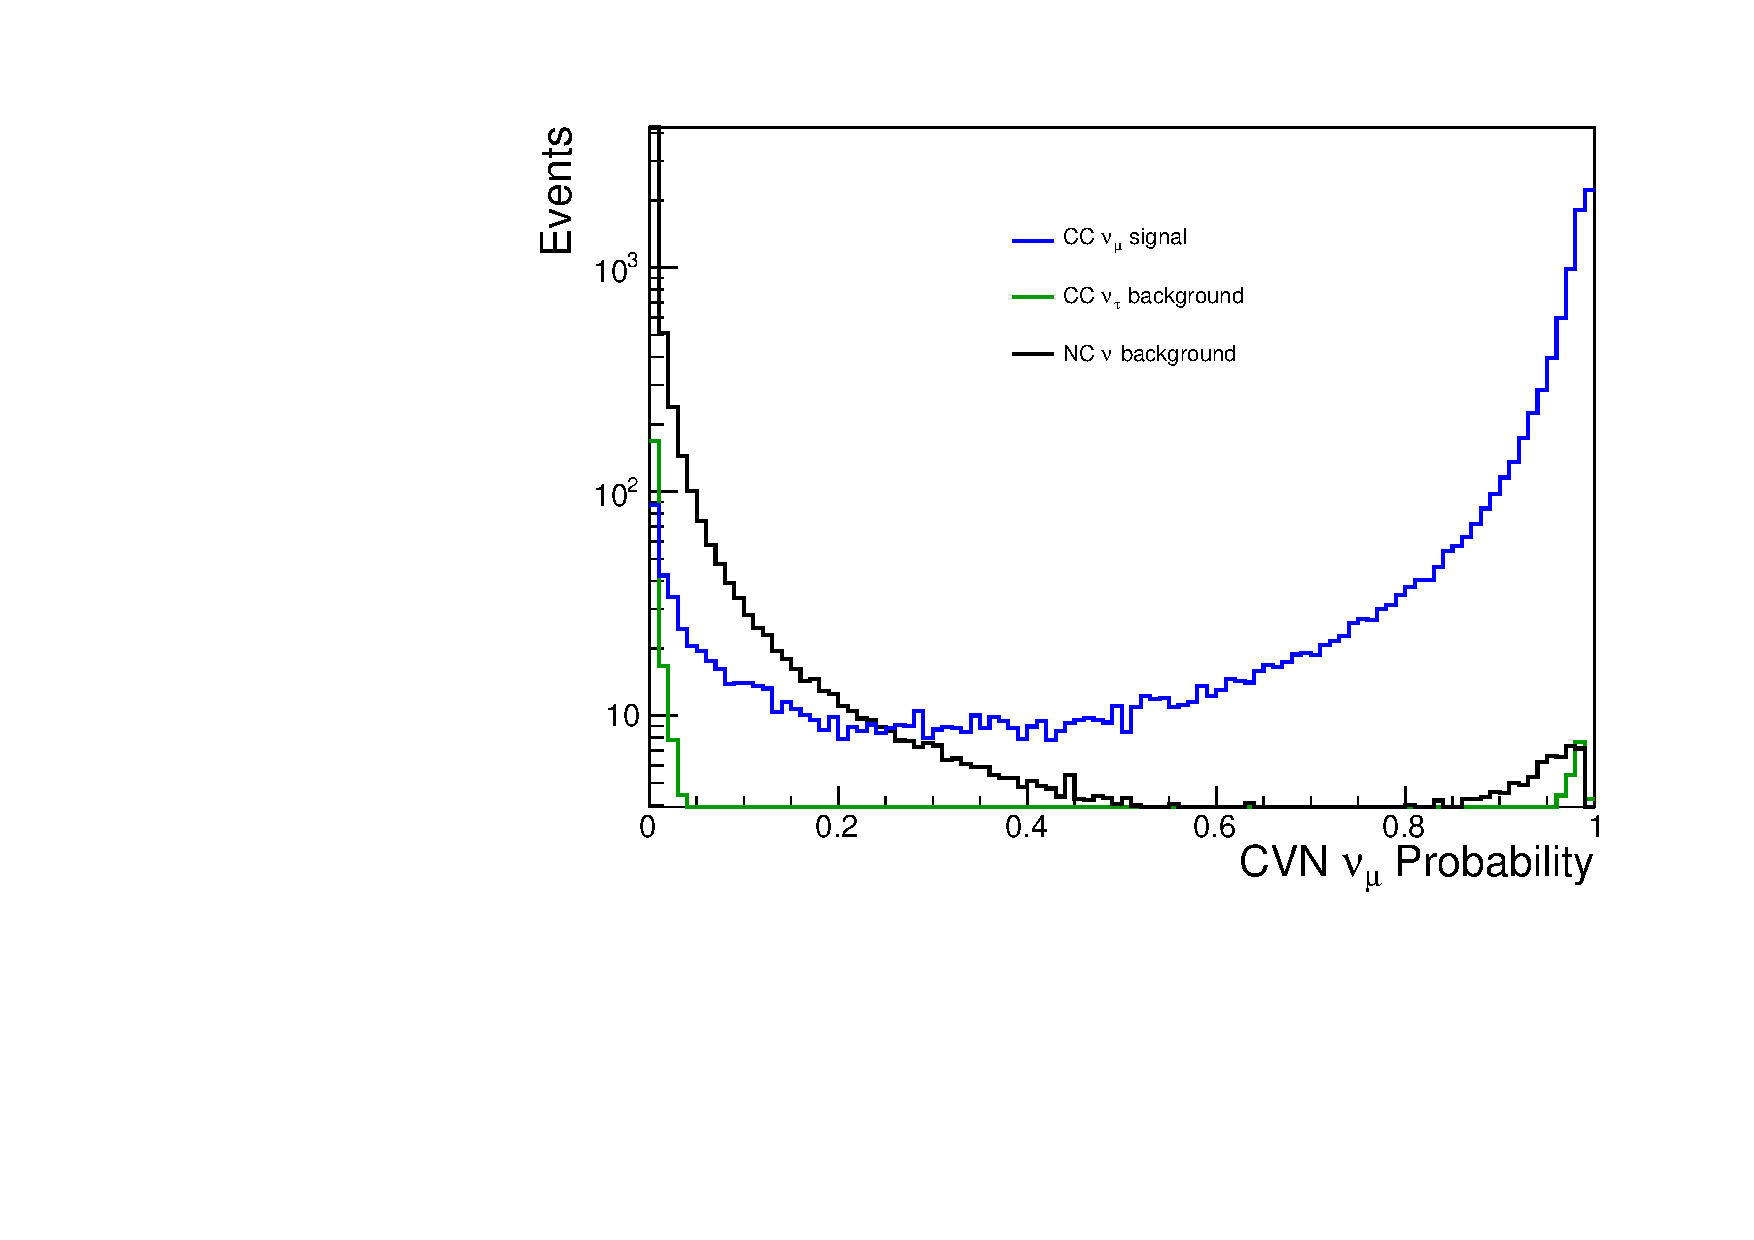
\includegraphics[width=0.45\linewidth]{cvn_numu_prob_log.pdf} 
	\end{tabular}
%	\caption{The neutrino flavour classification probabilities $P(\nu_e)$ (left) and $P(\nu_\mu)$ (right) for FHC-mode simulated CC$\nu_\mu$ (purple), CC$\nu_e$ (green), CC$\nu_\tau$ (cyan) and NC (orange) neutrino interactions.}
	\caption[The CVN \nue CC probability and \numu CC probability for the FHC beam mode]{The \dword{cvn} $\nu_e$ \dword{cc} probability (left) and $\nu_\mu$ \dword{cc} probability (right) for the \dword{fhc} beam mode shown with a log scale.}
    \label{fig:cvnprob}
\end{figure}

The $\nu_e$ \dword{cc} event selection uses events where $P(\nu_e \textrm{ \dword{cc}}) > 0.85$ for an interaction to be considered a candidate event of this type. Similarly, interactions are selected as $\nu_\mu$ \dword{cc} candidates if $P(\nu_\mu \textrm{ \dword{cc}}) > 0.5$. Note that since all of the flavor classification probabilities must sum to one, the interactions selected in the two event selections are completely independent. The same selection criteria are used for both \dword{fhc} and \dword{rhc} beam modes. The values used in the selection criteria were optimized to produce the best $\delta_{CP}$ sensitivity.

Figure~\ref{fig:nueeff} shows the efficiency as a function of reconstructed energy (under the electron neutrino hypothesis) for the $\nu_e$ event selection. The efficiency in both the FHC and RHC beam modes exceeds 90\% in the neutrino flux peak. %The good agreement with the selection efficiency from the \dword{dune} \dword{cdr}, which were developed using a parameterized detector response, provides reasonable confidence in the \dword{cvn} approach. 
Figure~\ref{fig:numueff} shows the corresponding excellent selection efficiency for the $\nu_\mu$ event selection.

\begin{figure}
    \centering
%    \begin{tabular}{cc}
		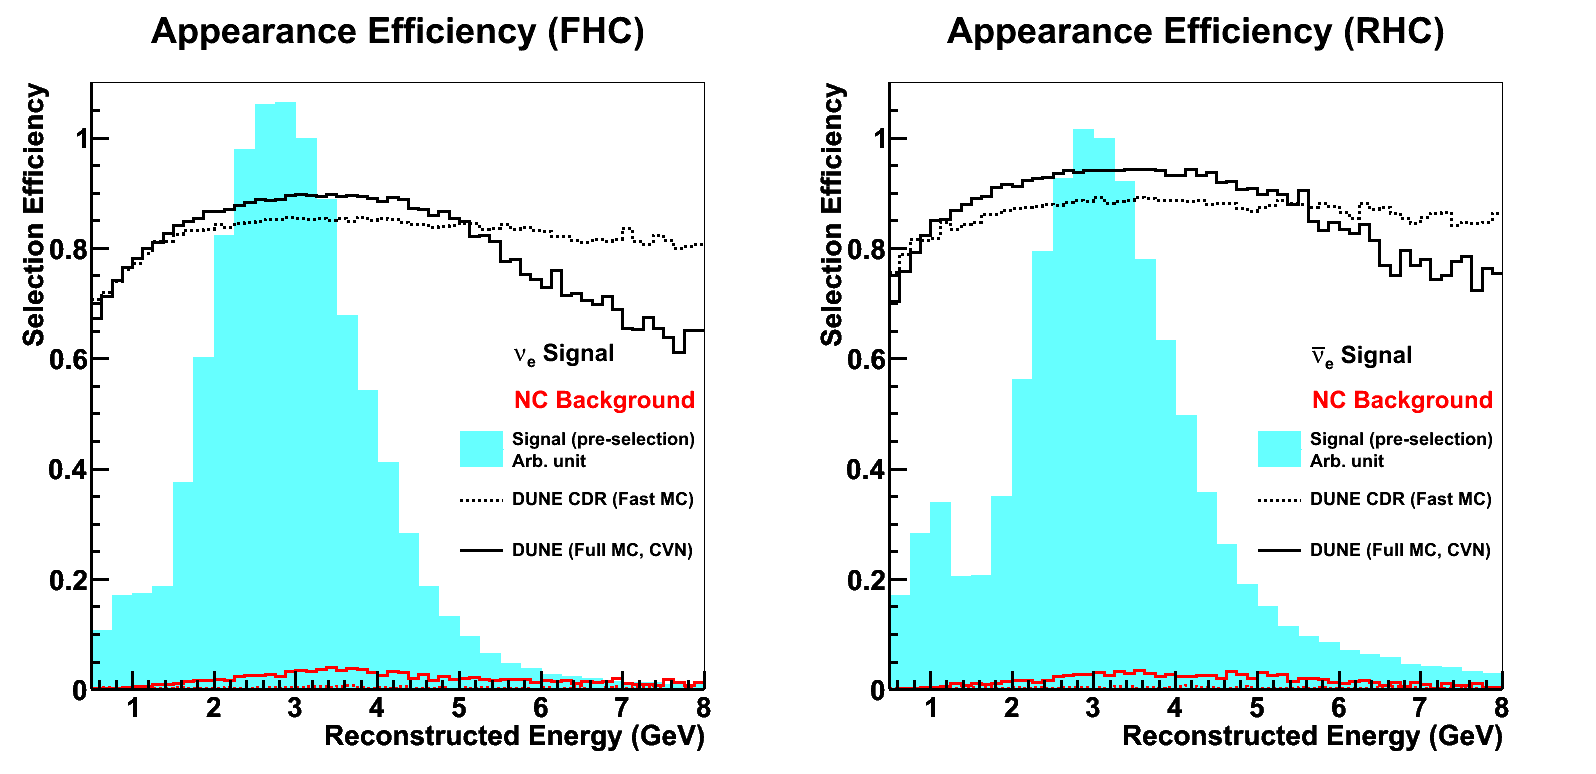
\includegraphics[width=0.9\linewidth]{cpv_compare_effs_cvnvcdr_dec2018_newcolor.png} %&
		%
\includegraphics[scale=0.22]{cvn_placeholder.pdf} 
%	\end{tabular}
	\caption[The $\nu_e$ CC selection efficiency for $P(\nu_e \textrm{CC}) > 0.85$]{The $\nu_e$ \dword{cc} selection efficiency for FHC-mode (left) and RHC-mode (right) simulation with the criterion $P(\nu_e \textrm{ \dword{cc}}) > 0.85$. The solid (dashed) lines show results from the \dword{cvn} (\dword{cdr}) for signal $\nu_e$ \dword{cc} and $\bar{\nu}_e$ \dword{cc} events in black and \dword{nc} background interaction in red. The blue region shows the oscillated flux (A.U.) to illustrate the most important regions of the energy distribution.}
    \label{fig:nueeff}
\end{figure}

\begin{figure}
    \centering
%    \begin{tabular}{cc}
		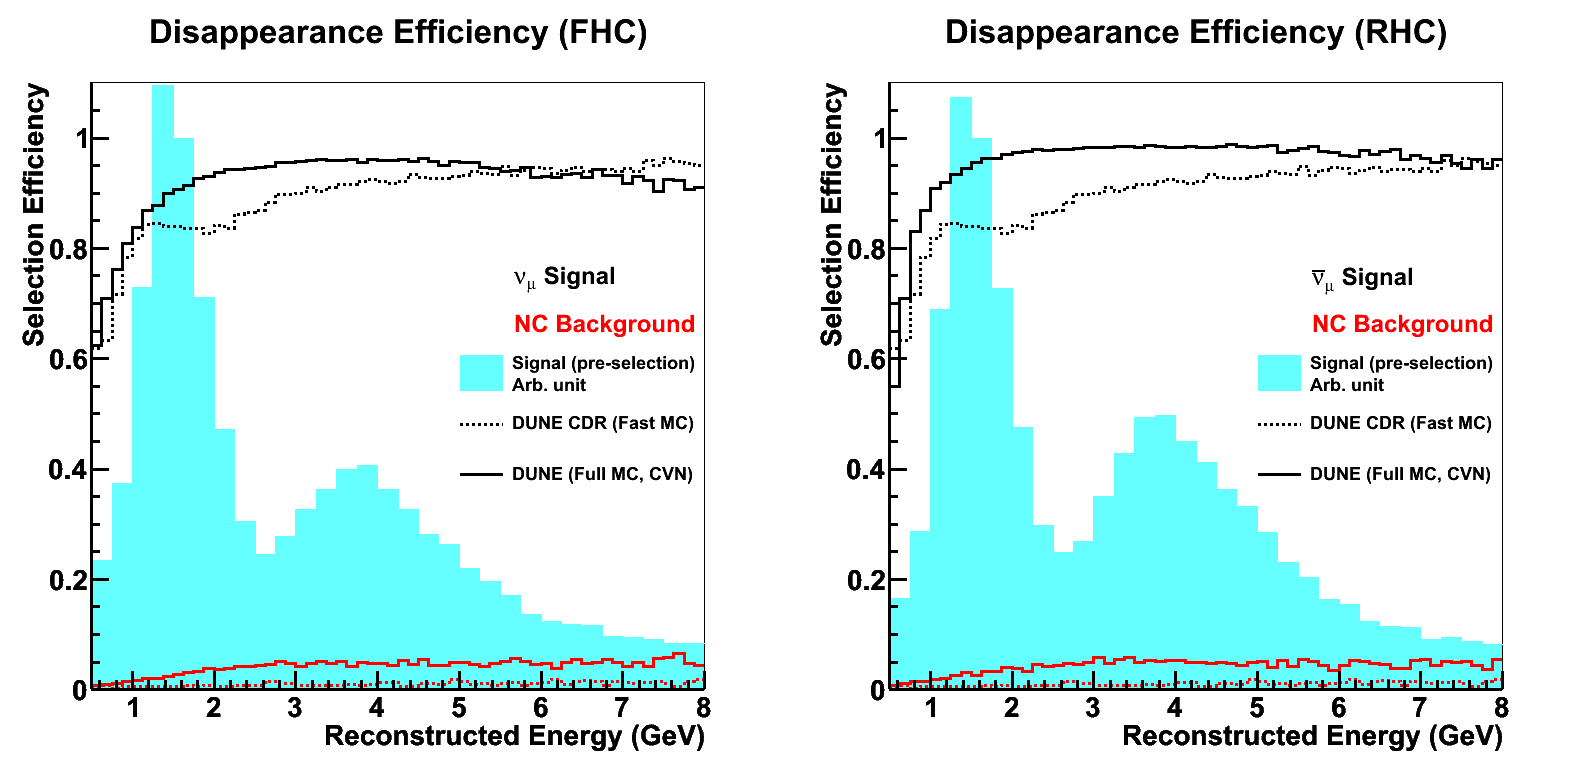
\includegraphics[width=0.9\linewidth]{cpv_compare_effs_dis_cvnvcdr_dec2018_newcolor.png} 
%	\end{tabular}
	\caption[The $\numu$ CC selection efficiency for $P(\numu \textrm{CC}) > 0.5$]{The $\numu$ \dword{cc} selection efficiency for FHC-mode (left) and RHC-mode (right) simulation with the criterion $P(\numu \textrm{ \dword{cc}}) > 0.5$. The solid (dashed) lines show results from the \dword{cvn} (\dword{cdr}) for signal $\numu$ \dword{cc} and $\bar{\nu}_\mu$ \dword{cc} events in black and \dword{nc} background interaction in red. The blue region shows the oscillated flux (A.U.) to illustrate the most important regions of the energy distribution.}
    \label{fig:numueff}
\end{figure}

%\subsubsection{Exclusive final states}
%The \dword{cvn} has four outputs that count the number of final-state particles for the following species: protons, charged pions, neutral pions and neutrons. Neutrino interactions with different final-state (after \dword{fsi}) particles can have varying energy resolutions due to differences in the complexity and particle multiplicity observed in the detector. The ability to accurately select exclusive final-states will allow for those interactions with very good energy resolution to be fully exploited in the oscillation fit to improve the sensitivity of the analysis. This information is not currently used in the analysis.

%The individual output probabilities from the \dword{cvn} can be multiplied together to give probabilities for exclusive selections. For example, Figure~\ref{fig:exclusive} shows the CC$\nu_\mu$ 1 proton probability on the left formed by the product 
%\begin{equation}
%P\left(\textrm{CC}\nu_\mu\,1\textrm{p}\right) = P\left(\textrm{CC}\nu_\mu \right) P\left( 1\,\textrm{p} \right) P\left( 0 \pi^\pm \right)P\left( 0 \pi^0 \right) P\left( 0\textrm{n} \right),
%end{equation}
%and the \dword{nc}$\pi^0$ probability on the right, defined similarly: 
%\begin{equation}
%P\left(\textrm{NC}\,1\pi^0\right) = P\left(\textrm{NC}\right) P\left(0\textrm{p} \right) P\left(0\pi^\pm \right) P\left(1\pi^0 \right) P\left( 0\textrm{n} \right).
%\end{equation}
%The background and signal distributions, closely peaked toward 0 and 1 respectively, demonstrate that the accurate selection of exclusive final states will be possible with the \dword{dune} \dword{cvn} technique. 

%\begin{figure}
%    \centering
%    \begin{tabular}{cc}
%		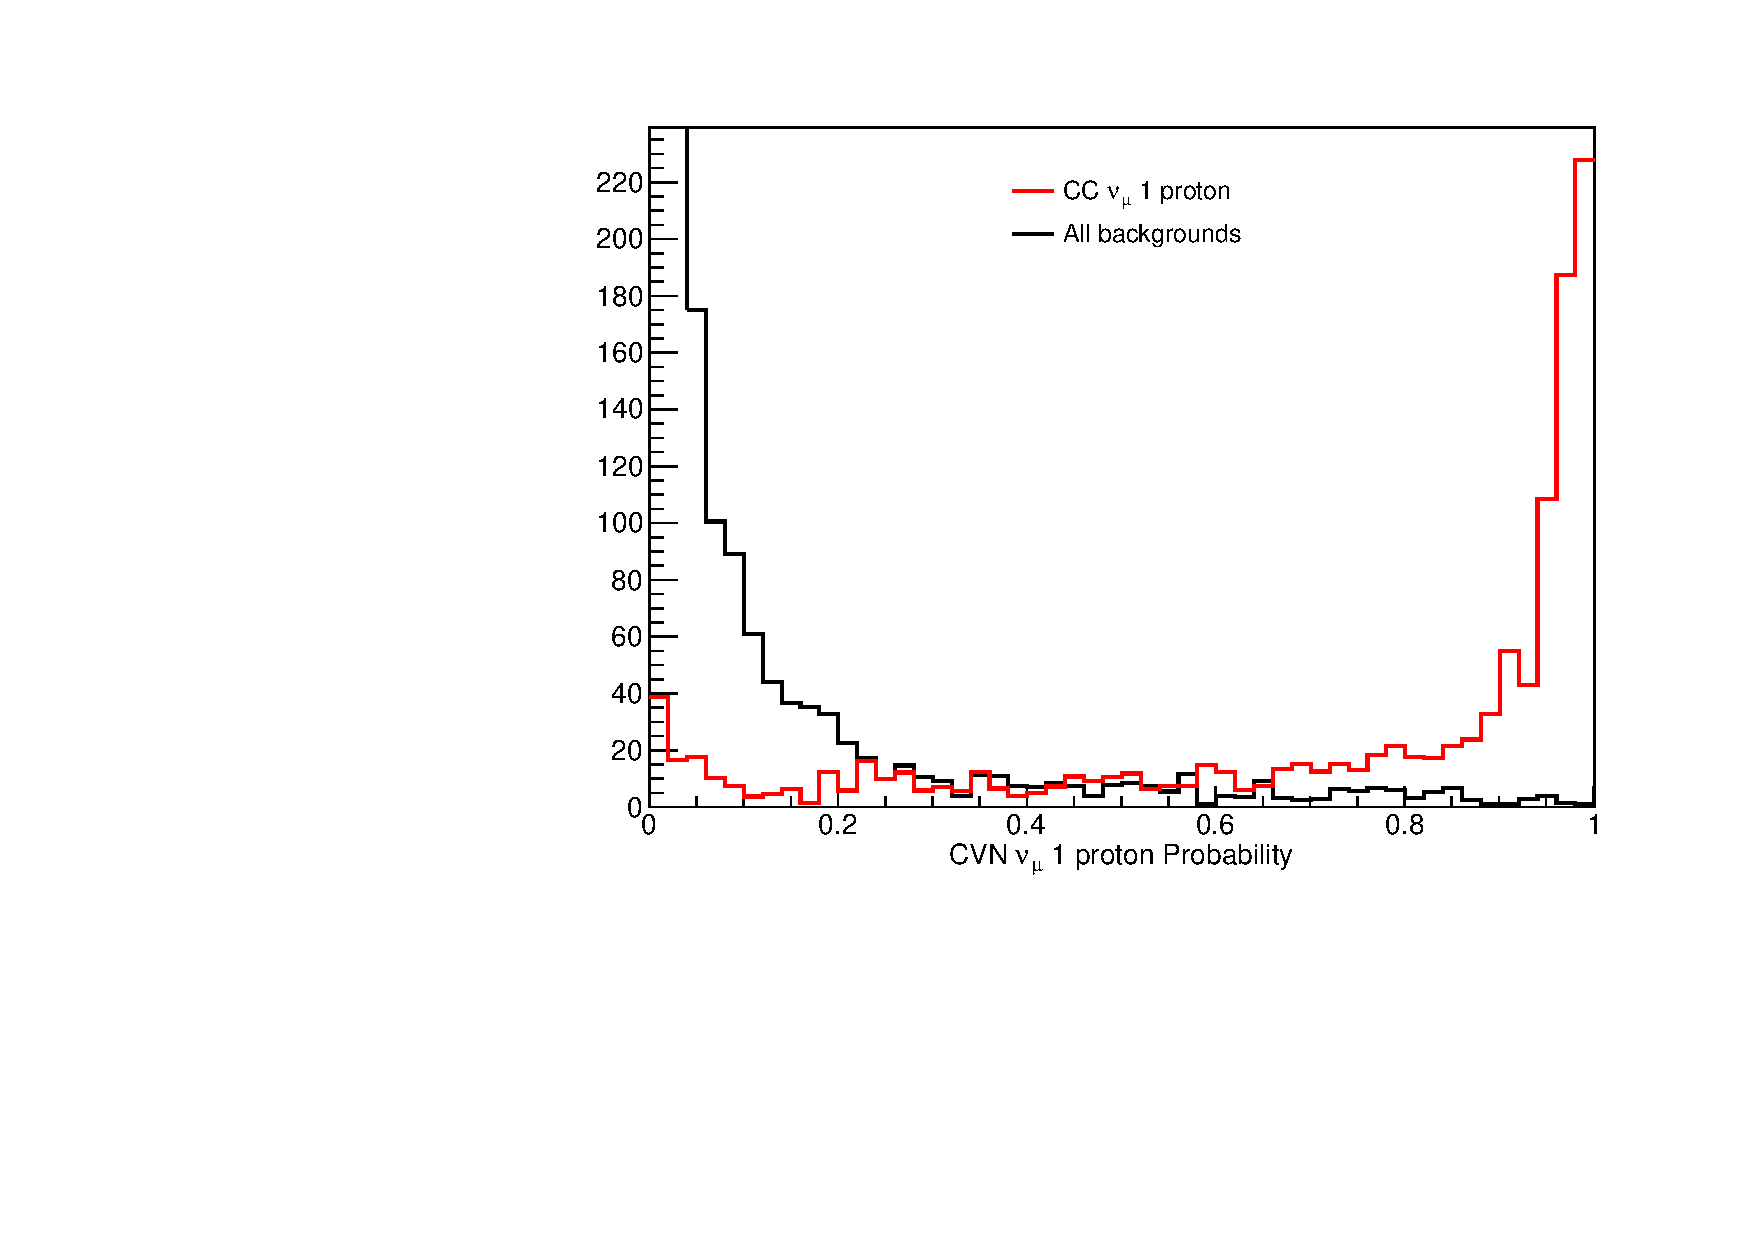
\includegraphics[width=0.475\linewidth]{ccNumu1ProtonProb.pdf} &
%		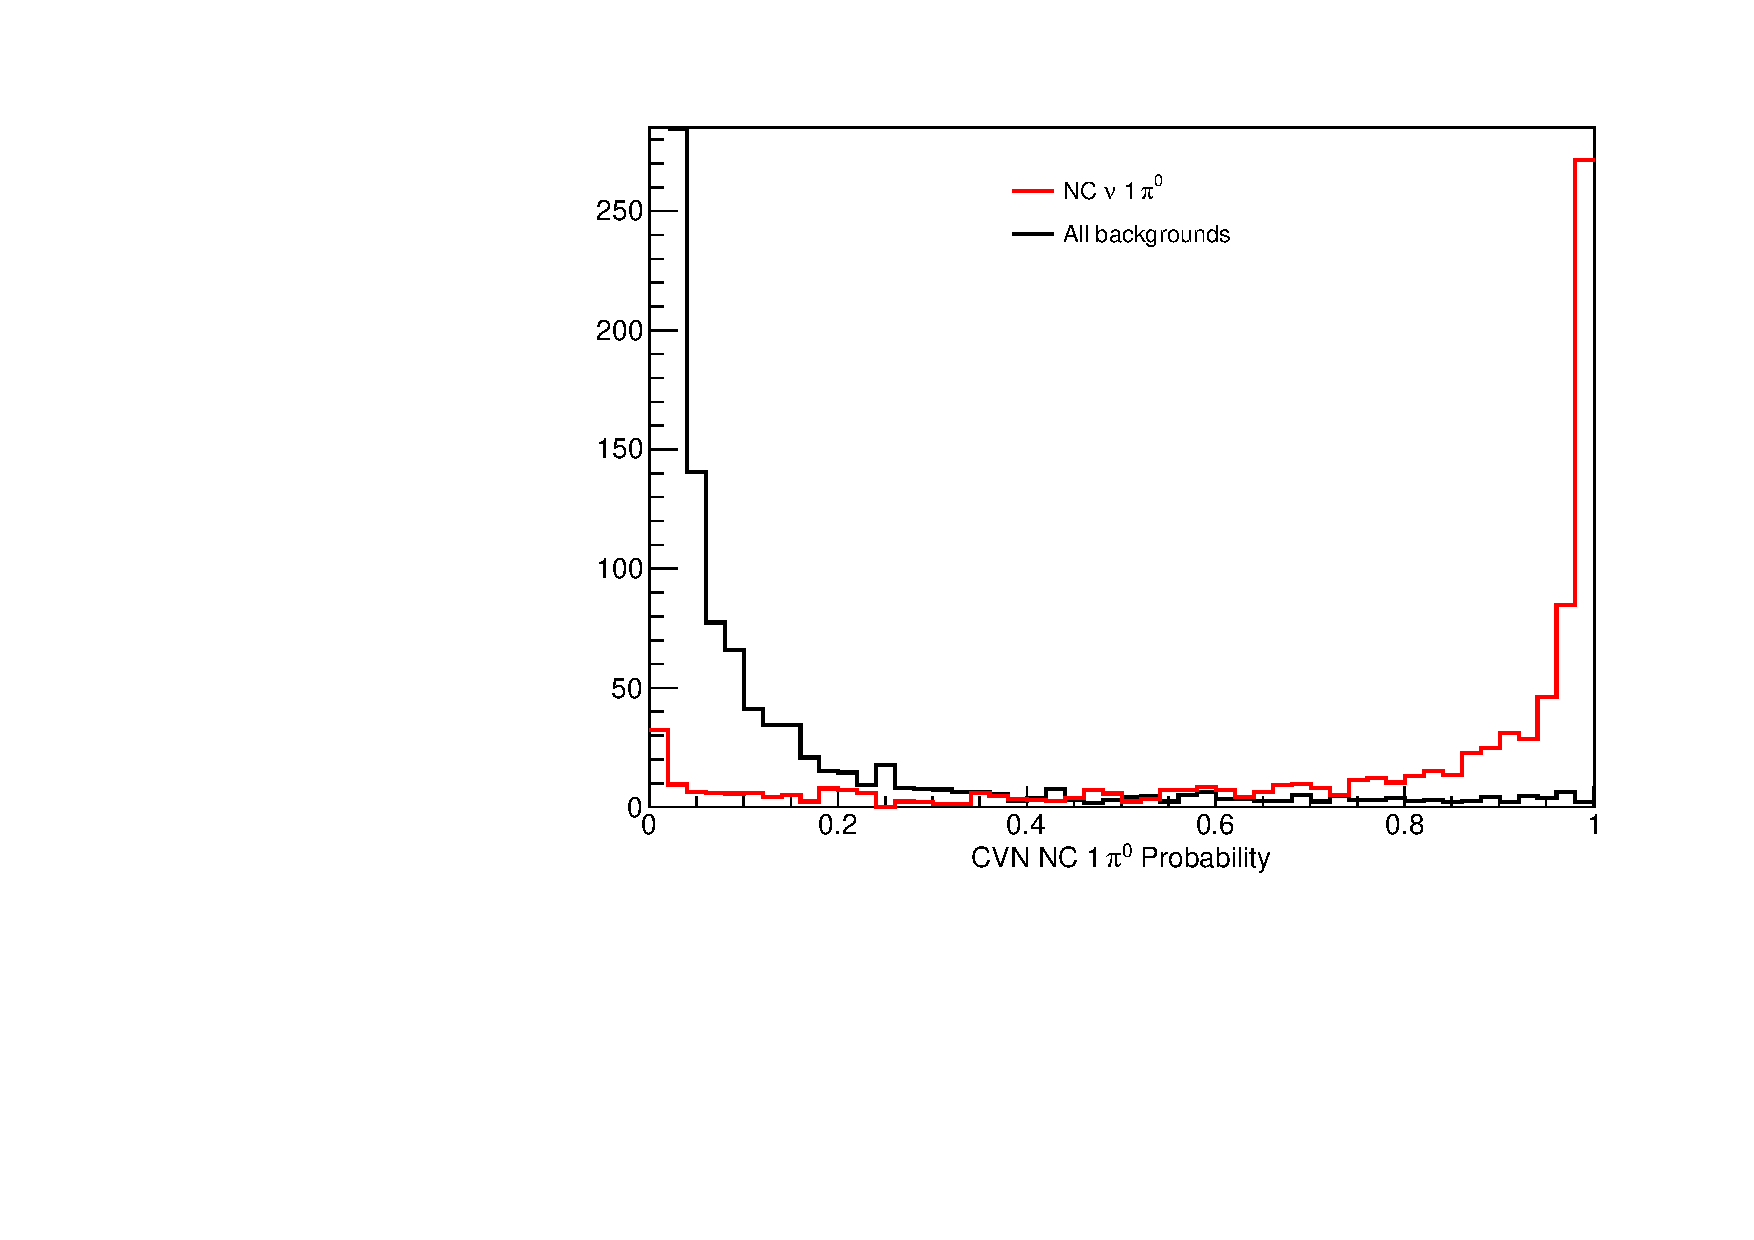
\includegraphics[width=0.475\linewidth]{nc1PizeroProb.pdf}
%	\end{tabular}
%	\caption{The \dword{cc}$\nu_\mu$ 1 proton (left) and \dword{nc} 1$\pi^0$ (right) probability distributions from the \dword{cvn}. In both cases the number of other particles is required to be zero.}
%    \label{fig:exclusive}
%\end{figure}

\subsubsection{Neutrino Flavor Identification Robustness}
A common concern on the applications of Deep Learning in high energy physics is the potential for differences in performance between data and simulation. Work is in progress to evaluate the \dword{dune} \dword{cvn} using data from a large \dword{dune} prototype, \dword{pdsp}~\cite{Abi:2017aow}.
%, collected data in a charged particle test beam at CERN in autumn 2018. Whilst there were no neutrino interactions, the data from \dword{pdsp} still provides the first important opportunity to compare the performance of the \dword{cvn} between data and simulation. Images can be created from individual reconstructed particles, including cosmic ray muons and test-beam electrons and positrons. For example, a cosmic ray muon image can mimic a simple \dword{cc}$\nu_\mu$ interaction, which can then be classified by the \dword{cvn}. The expected classification is \dword{cc}$\nu_\mu$ with no other final-state particle.%s, and the distribution of this probability is shown in Figure~\ref{fig:protodunecvn} for data and simulation. 
%While this work is in progress, initial results are promising, but are still very preliminary.
While the data-based validation is underway a thorough investigation of the selection efficiency as a function of various event kinematics was carried out. The results of the investigation is that that the \dword{cvn} selection does not suffer from model dependence at a level that would undermine the conclusions of the oscillation analysis studies. All efficiency curves are consistent with a few key observations. 

The ability of the \dword{cvn} to identify neutrino flavor is dependent on its ability to resolve and identify the charged lepton. %As charged lepton energy increases, and/or as hits from the charged lepton are masked by coincident energy depositions, efficiency decreases. 
Backgrounds are induced by mis-identification of charged pions for $\nu_{\mu}$ disappearance, and photons for $\nu_{e}$ appearance samples. Efficiency for these backgrounds tracks directly with the momentum and isolation of the energy depositions from the pions and photons. Efficiency was also observed to drop as a function of track/shower angle when energy depositions aligned with wire planes. The shapes of the efficiency functions in lepton momentum, lepton angle, and hadronic energy fraction (inelasticity) were all observed to be consistent with results from previous studies, including hand scans of \dword{lartpc} simulations. It is still conceivable that the efficacy is increased, especially at low charged lepton momentum, by the CVN identifying fine details of model dependent event kinematics. However, these effects are small enough to be covered by the assigned uncertainties. 



%\begin{figure}
%    \centering
%    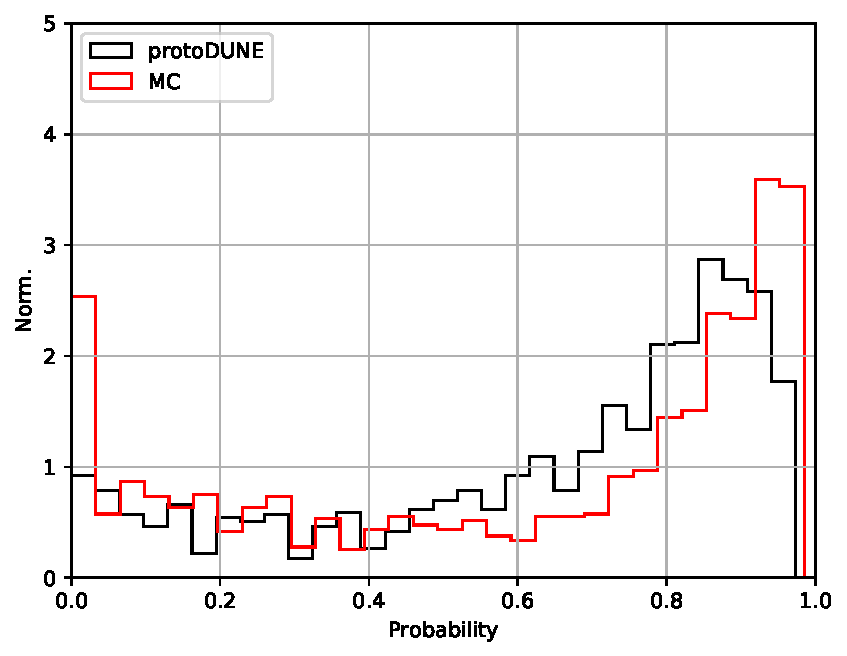
\includegraphics[scale=0.5]{cvn_protodata_mc.pdf}
%    
\includegraphics[scale=0.3]{cvn_placeholder.pdf}
    %\caption{Comparison of the \dword{cvn} response to cosmic ray muons in \dword{protodune} %data and simulation. TODO: this plot will be updated with a better plot after the next %round of \dword{protodune} data processing}
%    \label{fig:protodunecvn}
%\end{figure}

%While we are confident that any model dependent effects in the current \dword{cvn} are covered by uncertainties in the sensitivity studies, we also expect this possibility to be addressed before this technique would be used in any  analysis of DUNE data. 

Experience in ensuring robustness of deep learning image recognition techniques already exists within the community; similar techniques will be applied to future DUNE analyses. For example, the \dword{nova} experiment uses a technique that takes clear $\nu_{\mu}$ \dword{cc} interactions identified in data and simulation and removes all of the reconstructed hits associated with the reconstructed muon track. The reconstructed muon is replaced by a simulated electron with the same kinematic variables~\cite{Sachdev:2015hpa,Gandrajula:2018ytr}. This procedure was originally developed by \dword{minos}~\cite{Boehm:2009zz}, and allows a large sample of data-like electron neutrino interactions to be studied and excellent agreement was seen between the performance of the event selection for data and simulation. This approach will prove critical once \dword{dune} begins data taking to ensure the performance of the \dword{cvn} is the same for data and simulation.
%\fixme{citations NOvA_MRE and MINOS_MRE not found. anne}

\subsection{FD Neutrino Interaction Samples}

A complete neutrino interaction event simulation has been implemented, including realistic neutrino energy reconstruction and event selection algorithms which yields an appropriately accurate representation of the \dword{fd} samples to be used in the long-baseline oscillation analysis. The samples used in the sensitivity studies presented in this document require event by event simulations that effectively produce the convolution of the neutrino flux model, neutrino-argon scattering models, and models of the detector response. This last step must include estimates of energy smearing and bias, as well as the impact of a realistic event selection on signal acceptance and background rejection rates. This section has outlined the methods used to implement these algorithms. The final product is the  selected \dword{fd} event samples shown as a function of reconstructed neutrino energy in Section~\ref{sec:physics-lbnosc-osc}. Figure~\ref{fig:appspectra} shows the \numutonue and $\bar{\nu}_\mu \to \bar{\nu}_e$ appearance spectra and Figure~\ref{fig:disspectra} shows the \numutonumu and  $\bar{\nu}_\mu \to \bar{\nu}_\mu$ disappearance spectra. Tables~\ref{tab:apprates} and \ref{tab:disrates} provide the signal and background event rates for the appearance and disappearance analyses, respectively. Based on these predictions we observe the largest background to the \nue \dword{cc} appearance signal to be the intrinsic beam \nue interactions. There is also a contribution from misidentified neutral current interactions as well as small contributions from misidentified \numu and \nutau interactions. The \numu disappearance signal has negligible background, though there is a significant ``wrong-sign''  \numu component in the $\bar{\numu}$ sample. %The uncertainties on these predictions including those stemming from the detector response model, energy reconstruction and event selection algorithm are discussed in the next Section.

%ETW: Remove for now...may want to move some of this text to the systematics chapter
%\subsection{FD Systematics}
%\fixme{Expand/Write section as results are produced}
%FD systematics are those that affect the energy reconstruction (energy scale/bias, or energy resolution) or the efficiency. There are 3 categories of FD systematic being considered. The first is from interaction and FSI systematics. This is covered by the DUNErwt machinery, but the connection will be discussed here. The second is calibration uncertainties that will be based on input from the CalTF. This will also include the effects of inaccuracies from detector modelling (e.g. alignment) and detector failure modes (e.g. dead wires, electronics, etc.) Third is uncertainties on the detector model physics assumptions (i.e. GEANT4 uncertainties).  Currently Cafana is configured to fit energy scale and resolution systematics for the leptonic and hadronic components, as well as expanded FSI uncertainties in DUNErwt. These and other effects will also be explored by fake data (miscalibration effects via charge buildup, missing wire plains in various configurations, and moving energy in protons to neutrons are already planned). Explorations of the main source of GEANT4 errors will happen in the next couple weeks. Further discussion will have to wait for results on fitter development, and fitter performance evaluations during
%Hack Days (Nov 15-17). This development and evaluation will allow us to see which effects dominate and how, and thus must be discussed in detail, versus what has a small effect and can be discussed briefly.


% End DUNE CVN event selection subsection

% \subsubsection{Simulation and Reconstruction Parameters}
% \subsubsection{Energy Reconstruction}
% \begin{itemize}
% \item New plots: Smearing matrices (Update to include latest Ereco)
% \item New plots: Muon, shower, hadronic, neutrino energy resolution and bias  (Update to include latest Ereco)
% \end{itemize}

% \subsection{Event Selections and Spectra}
% Descriptions and plots of efficiency, purity, sig/bkg discriminants, spectra for each selection:
% \begin{itemize}
% \item MVA Selections (Update to latest version)
% \item Pandora-based PID Selections (Update to latest version)
% \item CVN Selections (Update to latest version)
% \end{itemize}

% Tables:
% \begin{itemize}
% 	\item CDR Table 3.5: Nue/Nuebar appearance rates
% 	\item CDR Table 3.6: Numu/Numubar disappearance rates
% \end{itemize}